\chapter{Experimentation \& Evaluation}
This chapter focuses on the evaluating the experiments with each agent, and the
results obtained doing so. We analyse the reasoning behind the results, and
propose potential mechanisms to improve them. The architecture of the neural
networks was kept relatively constant throughout the process, as this was not
the basis of the experiments.

\section{Hyperparameter Selection}

Due to the hyperparameter sensitivity of the deep Q-network (DQN) and the
advantage actor-critic (A2C) algorithm, paired with the long training time for
the agents, experimentation required a wealth of thought and effort channeled
precisely towards the correct direction. As mentioned in the abstract, the aim
of this project was to reduce training time, so we make comparisons using the
results after training the agents for 500 episodes. All of the hyperparameters
used in the algorithms are provided in \autoref{chp:hyperparameters}.

The learning rates for the all of the networks except the Car Racing A2C were
kept at $1\times 10^{-3}$; this value was found to produce relatively fast
convergence without compromising too much on the stability. For the Car Racing
A2C agent, this value was found to be too high; the agent would quickly
converge to the "gas" for all of the states as a "master action", so the
learning rate was set to $1\times 10^{-5}$.

A critical hyperparameter for the deep Q-learning algorithm was the
$\epsilon$-decay multiplier; we found that a value of 0.99 struck the balance
between enough exploration, while still allowing the agent to exploit its
discovered strategies enough within 500 episodes.

Although it has been found that large batch sizes improve training performance
\cite{stooke2018accelerated}, this would require high end compute resources,
especially a lot of memory and CPU cache. Due to this constraint, we found the
maximum batch size of 32 for the deep Q-learning algorithm to be high enough to
train the agent without negatively impacting quality substantially, while being
low enough to not crash the training machine due to excessive resource usage.

\begin{table}[H]
  \centering
  \begin{tabular}{|c|c|c|c|}
    \hline
    \multicolumn{2}{|c|}{\multirow{2}{*}}                        & \multicolumn{2}{c|}{\textbf{Game}}                                                                             \\
    \cline{3-4}
    \multicolumn{2}{|c|}{\multirow{-2}{*}{\textbf{Score Table}}} & \textbf{Mountain Car}                                                & \textbf{Car Racing}                     \\
    \hline
    \multirow{4}{*}{\textbf{Agent}}
                                                                 & \textbf{Random}                                                      & $-200\pm 0$         & $-65\pm 6$        \\
                                                                 & \textbf{DQN}                                                         & $-137\pm21$         & $\bm{623\pm 182}$ \\
                                                                 & \textbf{A2C}                                                         & $\bm{-135\pm 32}$   & $-17\pm 47$       \\
                                                                 & \textbf{Research} \cite{hernandez2019understanding, ha2018recurrent} & $-151 \pm 18$       & $343 \pm 18$      \\
    \hline
  \end{tabular}
  \caption[DQN and A2C testing results]{Average rewards after 500 episodes of training (1000 episode testing mean). The highest score for each game is in \textbf{bold}.}
  \label{table:results}
\end{table}


\section{Mountain Car}

\subsection{Model Evaluation}

As we can see from the rolling mean reward graph in
\autoref{fig:mountain_car_rewards}, both algorithms start to converge to a
solution by 500 episodes. A2C initially learns much quicker than the DQN, but
the DQN catches up by 450 episodes.

\begin{figure}[H]
  \centering
  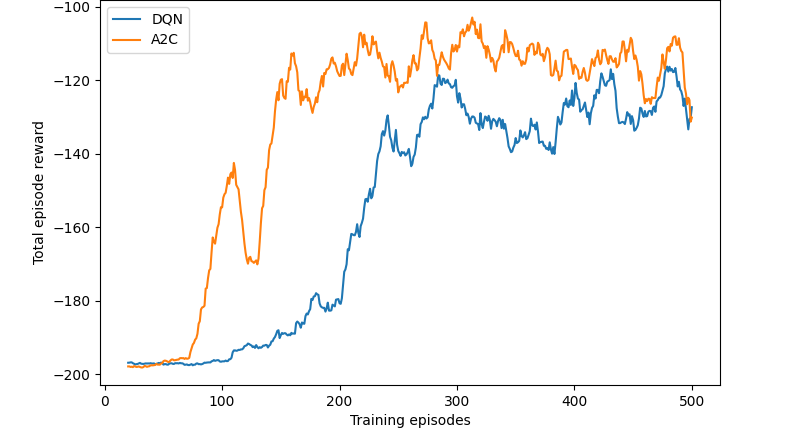
\includegraphics[width=0.75\textwidth]{figures/images/mountain_car_rewards.png}
  \caption[Mountain Car training rewards]{Mountain Car training rewards for DQN and A2C agents, with 20 episode rolling average}
  \label{fig:mountain_car_rewards}
\end{figure}


The first column in \autoref{table:results} shows the average scores for the
Mountain Car agents with 1000 test episodes; both of the algorithms perform
extremely similarly in terms of raw score. They both greatly outperform both
the research value and random action\footnote{This is the score of an agent
  that chooses completely random actions} value by over 13 points, which equates
to approximately a 9\% improvement in score. The standard deviation in the
score for the DQN agent is very similar to the research value; the same can not
be said about the A2C agent, which displays approximately a 50\% higher
standard deviation compared to the research and DQN values. This indicates that
the DQN is more confident in its policy, while the A2C is much less stable.

\subsection{Visualization Evaluation}
For Mountain Car, the visualization presents a histogram of the neural
network's weights as shown in \autoref{fig:mountain_car_w_viz}, and a line
graph with the weights values from one node to all of it's connected nodes as
shown in \autoref{fig:mountain_car_n_viz}. These are the middle layer's weights
for the deep Q-network and the A2C's actor network. They can be controlled
using a slider, to use a snapshot of the network at the selected the number of
training episodes. In \autoref{fig:mountain_car_w_viz} and
\autoref{fig:mountain_car_n_viz}, we can see the progression of the neural
network from 25 training episodes to 500; the network's improvement is clear,
from randomly selecting actions as the weights are relatively uniformly spread,
to wider distribution of a few weights with a high density of weights around 0
indicating learned features.

\begin{figure}[H]
  \captionsetup[subfigure]{justification=centering}
  \centering
  \begin{subfigure}[t]{0.47\linewidth}
    {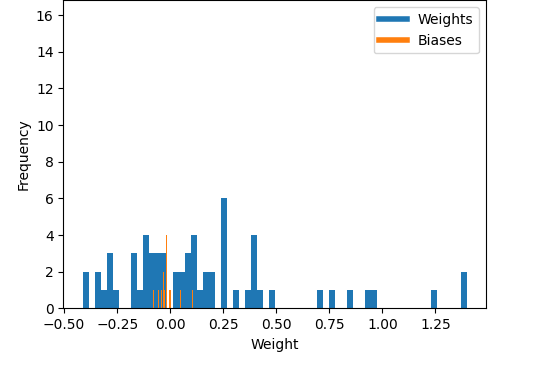
\includegraphics[height=5cm]{figures/images/mountain_car_weights_25.png}}
    \caption{After 25 episodes}
  \end{subfigure}
  \hfill
  \begin{subfigure}[t]{0.47\linewidth}
    {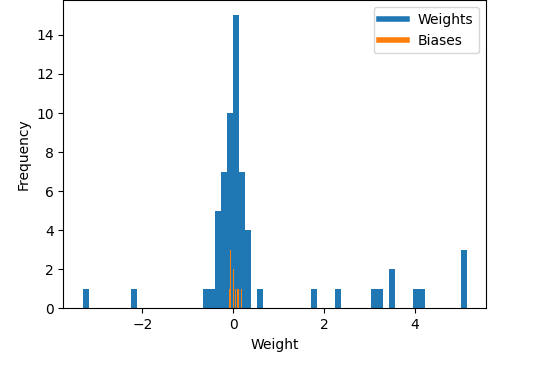
\includegraphics[height=5cm]{figures/images/mountain_car_weights_500.png}}
    \caption{After 500 episodes}
  \end{subfigure}
  \caption{Mountain Car weight distribution graphs}
  \label{fig:mountain_car_w_viz}
\end{figure}


\begin{figure}[H]
  \captionsetup[subfigure]{justification=centering}
  \centering
  \begin{subfigure}[t]{0.47\linewidth}
    {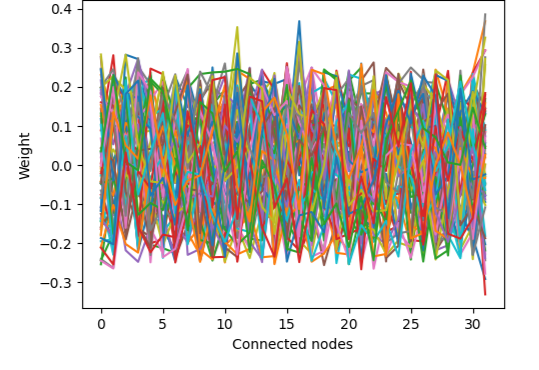
\includegraphics[height=5cm]{figures/images/mountain_car_nodes_25.png}}
    \caption{After 25 episodes}
  \end{subfigure}
  \hfill
  \begin{subfigure}[t]{0.47\linewidth}
    {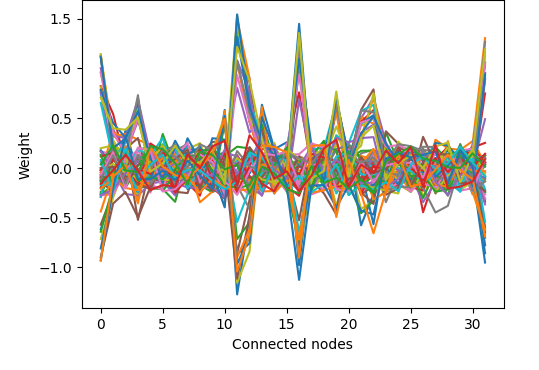
\includegraphics[height=5cm]{figures/images/mountain_car_nodes_500.png}}
    \caption{After 500 episodes}
  \end{subfigure}
  \caption{Mountain Car node connection graphs}
  \label{fig:mountain_car_n_viz}
\end{figure}


\subsection{Gameplay Findings}

Viewing the gameplay indicated which actions the agents were taking; it was
observed that both agents would accelerate too much towards the left and bump
into the environment boundary, instead of reversing acceleration earlier on the
hill. This is likely a result of the reward shaping function defined in
\autoref{sec:reward_shaping}, as it always promotes increasing speed without
consideration for the agent's position. An optimization would be a more nuanced
reward function, that for example disincentivizes speeds over a certain
threshold when the agent's state is on the left hill.

\subsection{Catastrophic Forgetting}

At around 100 episodes, the A2C agent's score suddenly drops by a substantial
amount, as we can see in \autoref{fig:mountain_car_rewards}. This is likely due
to the phenomenon of catastrophic forgetting \cite{parisi2019continual}, which
happens because the agent drastically updates the weights in the network when
learning a new strategy because of exploring new experiences. Mitigating this
issue could involve an approach such as implementing progressive neural
networks \cite{rusu2016progressive} or dynamic self-organizing maps
\cite{lo2019overcoming}.

\subsection{Exploration Action Probabilities}

A major revelation for the DQN agent was setting a custom probability
distribution for the $\epsilon$-greedy exploration; instead of sampling the
action from a uniform distribution, we specified an array with the probability
for each action which allowed exploration to be biased towards actions that
usually lead to higher rewards; in this case, that is the "left" and "right"
actions rather than doing nothing. We can find the custom probability
distribution for the Mountain Car actions in
\autoref{table:mountain_car_dqn_probs}.

\begin{table}[H]
  \centering
  \begin{tabular}{|c|c|c|c|c|c|c|}
    \hline
    \textbf{Action}      & Left & Nothing & Right \\
    \hline
    \textbf{Probability} & 0.4  & 0.2     & 0.4   \\
    \hline
  \end{tabular}
  \caption{Mountain Car DQN action probabilities} \label{table:mountain_car_dqn_probs}
\end{table}


Since we are not using an $\epsilon$-greedy policy for the advantage
actor-critic algorithm, the same distribution could not be applied to it.

\section{Car Racing}

\subsection{Model Evaluation}

The complexity of this environment posed a challenge to both of the algorithms,
though the A2C agent struggled more to start converging to a policy; as we can
see in \autoref{fig:car_racing_rewards}, the DQN just starts to converge by the
end of the 500 training episodes, as the variation in episode rewards starts to
decrease slowly. However, the A2C agent is severely lagging behind; it was
trained for longer to ensure there wasn't a fault in the algorithm, and it
started improving in performance by 750 episodes.

\begin{figure}[H]
  \centering
  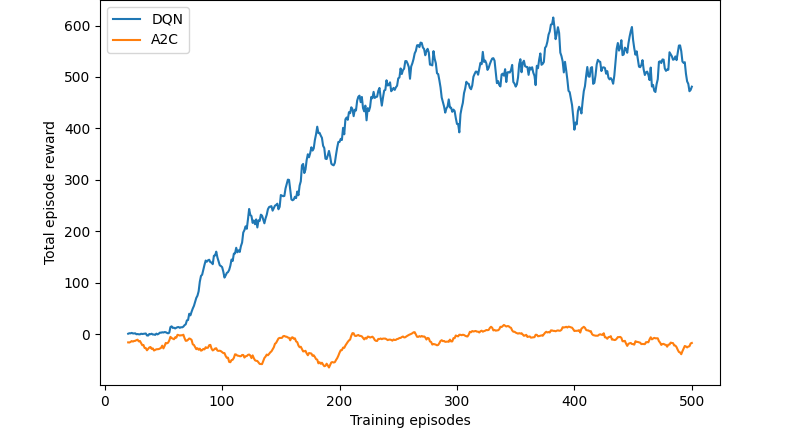
\includegraphics[width=0.75\textwidth]{figures/images/car_racing_rewards.png}
  \caption[Car Racing training rewards]{Car Racing training rewards for DQN and A2C agents, with 20 episode rolling average}
  \label{fig:car_racing_rewards}
\end{figure}


The second column in \autoref{table:results} shows the average scores for the
Car Racing agents with 1000 test episodes; the DQN agent far outperforms all of
the other agents, including the A2C agent, the research value and the random
action value. It must also be noted that the standard deviation for the DQN
agent is far higher than any of the others, indicating that the training is
still very unstable, and that the agent hasn't fully converged to an optimal
Q-function. Looking at final scores, the DQN agent outperforms the research
value approximately 86\%; while the A2C agent doesn't reach this score within
500 episodes, it performs as well as the DQN agent after 1000 episodes.

One reason why the A2C algorithm takes longer to converge could be due to the
one-step nature of the algorithm. We define a custom reward function for
Mountain Car, so it's not a problem in that environment, but one-step lookahead
severely limits the capability of Car Racing agent. The benefit to looking
ahead further to compute the expected return is that it would allow the agent
to make moves based on longer term changes in the track, such as a corner "out
of sight" for the one-step algorithm.

\subsection{Visualization Evaluation}
For Car Racing, the visualization shows the progression of the filters from the
first convolution layer of the network; in the case of the A2C agent, it shows
the actor's filters. In \autoref{fig:car_racing_filter_viz}, we can see the
change in the CNN filters; the vertical axis represents the filter, and the
horizontal represents which frame in the frame stack the filter corresponds to.
While slightly less informative than the visualization for Mountain Car, it is
still indicative of the change in the filters after training. We can also see
these filters applied to a frame of the game, in
\autoref{fig:car_racing_frame_viz}; this shows the filters' corresponding
feature maps\footnote{Note that the feature map visualization was not included
  in the final code submission}, where the road is clearly distinguished from the
rest of the image. Similarly to the Mountain Car visualization, a slider can be
used to select the number of episodes to determine which neural network to use.

\begin{figure}[H]
  \captionsetup[subfigure]{justification=centering}
  \centering
  \begin{subfigure}{0.44\linewidth}
    {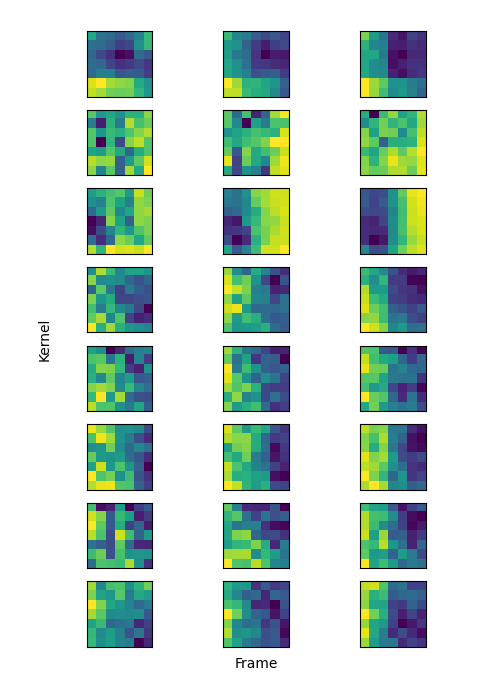
\includegraphics[height=9cm]{figures/images/car_racing_filters_25.png}}
    \caption{After 25 episodes}
  \end{subfigure}
  \hfill
  \begin{subfigure}{0.44\linewidth}
    {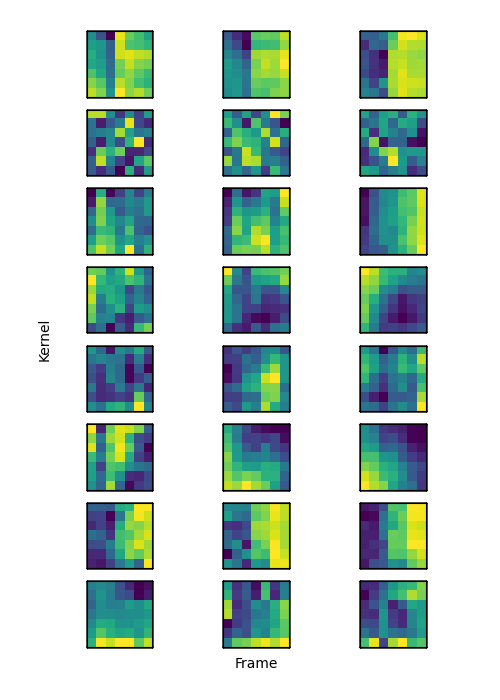
\includegraphics[height=9cm]{figures/images/car_racing_filters_500.png}}
    \caption{After 500 episodes}
  \end{subfigure}
  \caption[Car Racing filter plots]{Car Racing layer 1 filter plots}
  \label{fig:car_racing_filter_viz}
\end{figure}


\begin{figure}[H]
  \captionsetup[subfigure]{justification=centering}
  \centering
  \begin{subfigure}{0.44\linewidth}
    {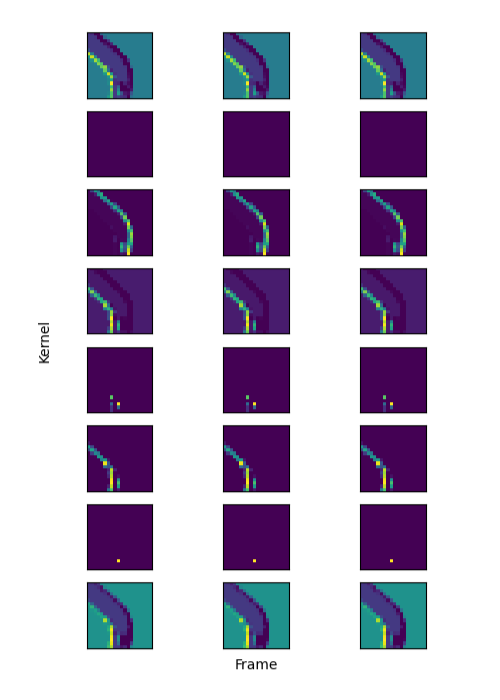
\includegraphics[height=9cm]{figures/images/car_racing_frames_25.png}}
    \caption{After 25 episodes}
  \end{subfigure}
  \hfill
  \begin{subfigure}{0.44\linewidth}
    {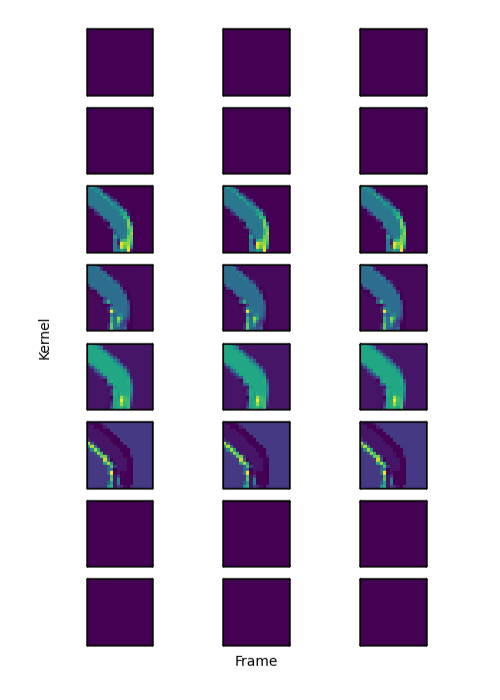
\includegraphics[height=9cm]{figures/images/car_racing_frames_500.png}}
    \caption{After 500 episodes}
  \end{subfigure}
  \caption[Car Racing feature map plots]{Car Racing layer 1 feature map plots}
  \label{fig:car_racing_frame_viz}
\end{figure}


\subsection{Gameplay Findings}
The gameplay for Car Racing was very insightful; as training progressed, the
agents learned to cut sharp corners, but they also started to very slowly veer
off the edge of the track, losing points. The main reason the agents couldn't
complete the track was spinning out of control, and they would usually not
recover from this. They would end up on a part of the environment with only
grass, or if they found their way back to the track, they would not know which
way was forward as there is no indication of direction in the environment. This
can be mitigated by training for more than 500 episodes, as the agents would
reach a more stable and optimal policy.

\subsection{Negative Reward Break}
A major finding during experimentation was that the episodes would last
extremely long, with the agent's consistently losing points, especially in the
early stages of training. To mitigate this issue, a negative reward break was
implemented. If the agent receives a negative reward consecutively for a
threshold number of steps, the episode is terminated.

A threshold value of 100 was found to provide a balance between the episodes
not lasting too long, and the agent learning to recover from minor errors that
would result in a few steps of consecutive negative rewards.

\subsection{Exploration Action Probabilities}
Similarly to the DQN used for Mountain Car, biasing the agent towards certain
actions helped in the training speed of the algorithm. The car benefits from
exploring the "gas" action the most, which is expected as it needs to move
forward to pass more tiles on the track. We can find the custom probability
distribution for the Car Racing actions in
\autoref{table:car_racing_dqn_probs}.

\begin{table}[H]
  \centering
  \begin{tabular}{|c|c|c|c|c|c|c|}
    \hline
    \textbf{Action}      & Nothing & Left & Right & Gas & Brake \\
    \hline
    \textbf{Probability} & 0.0     & 0.2  & 0.2   & 0.5 & 0.1   \\
    \hline
  \end{tabular}
  \caption{Car Racing DQN action probabilities}
  \label{table:car_racing_dqn_probs}
\end{table}


\subsection{Frame Skipping}
With the highly dynamic and fast-paced nature of this environment, the commonly
used value in research of skipping $n = 3$ frames \cite{bellemare2013arcade}
turned out to be too high; the agent would go off course by repeating the same
move for too long, due to the high speed of the car. A value of skipping $n =
  2$ frames yielded the optimal balance between reducing correlative frame data
without overextending the single chosen action. Note that reward was still
measured for the skipped frames, and used by the agent in training the
networks.
